
\section{Motivating Example}

In this section, we introduce a real world \BPG{} for management of sepsis
in pediatric cases to motivate the need for Guidelines-based Clinical Decision Support Systems,
and to illustrate characteristics that are desired of a framework for building
\CDSSs{}.
Sepsis is life-threatening condition caused by the body's extreme response to
an infection \cite{RhodesICM17}, and is
a major cause of morbidity and mortality in children \cite{Eisenberg2021JP}.
Adverse outcomes can, however, be mitigated through timely
identification and prompt treatment with antibiotics and
intravenous (IV) fluids \cite{Weiss2014CCM,Evans2018JAMA}.
\BPGs{} for screening and management of sepsis in pediatric Emergency
Departments (EDs) have shown effectiveness in screening and management of sepsis \cite{Eisenberg2021JP},
leading to their adoption in many pediatric EDs \cite{Balamuth2017EM,Sepanski2014FP}.



\begin{figure}[t]
  \centering
  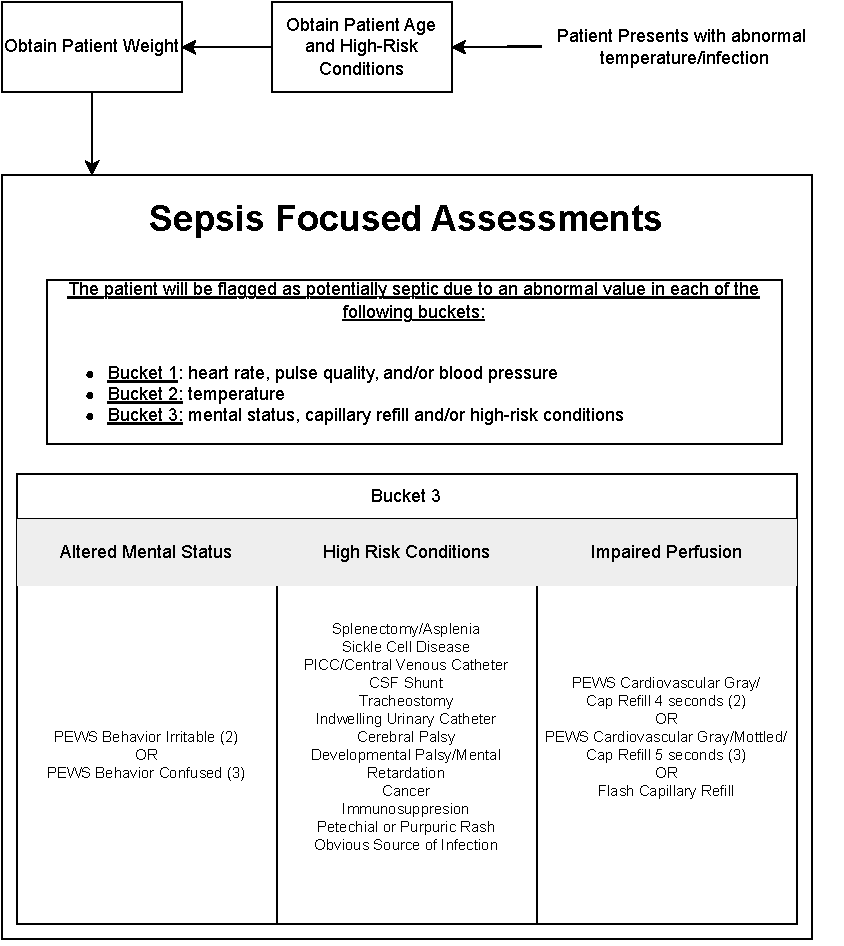
\includegraphics[width=0.45\textwidth]{sepsis-screening-osf}
  %\includegraphics[width=0.5\textwidth]{screening-vitals}
  \caption{Pediatric sepsis screening \BPG{}}\label{fig:sepsis-screening}
\end{figure}

In \figurename{} \ref{fig:sepsis-screening}, we present a simplified version of
the screening section of OSF's sepsis management guideline.
In essence, when a patient arrives at the
\ED{} with a fever or an infection, the \HCP{} is supposed to obtain
\begin{enumerate*}[label=(\alph*)]
  \item the patient's age,
  \item any conditions, such as cancer, immunosuppresssion, etc,
    that increase likelihood of sepsis, and
  \item the patient's vital signs, such as heart rate, systolic blood
    pressure, respiratory rate, etc.
\end{enumerate*}
This information is then used to check for abnormalities
in clusters of linked information, called \say{buckets}. For instance, if
the patient's heart rate is abnormal, then \say{bucket 1} is said to
have an abnormal value.
Checking for such abnormalities often involves the use of tables, such as
\tablename{} \ref{table:vital-signs}, that contain normal ranges indexed by
\emph{age}.
%\footnote{For brevity, we omit some age ranges and vital signs from table
%\ref{table:vital-signs}}.
If the patient has at least one abnormal value in every \say{bucket},
then he/she is flagged as potentially septic.


The \BPG{}-recommended treatment for
sepsis involves multiple concurrent workflows, such as
screening for septic shock, fluid resuscitation, and administering antibiotics.
In \figurename{} \ref{fig:fluid-therapy}, we provide
a version of the fluid resuscitation guideline used
at OSF. Briefly, if the patient is flagged as potentially septic, the guideline suggests
\begin{enumerate*}[label=(\roman*)]
  \item obtaining any fluid-overload risks,
  \item administering normal saline (typically over a period of 15 minutes),
    where the dosage is dictated by risks determined in previous step,
  \item assessing signs of fluid-overload,
  \item evaluating patient responsiveness to normal saline upon completion of
    the administering process, and,
  \item determining whether another fluid bolus should be administered based on
    information from previous steps.
\end{enumerate*}
\begin{figure}[b]
  \centering
  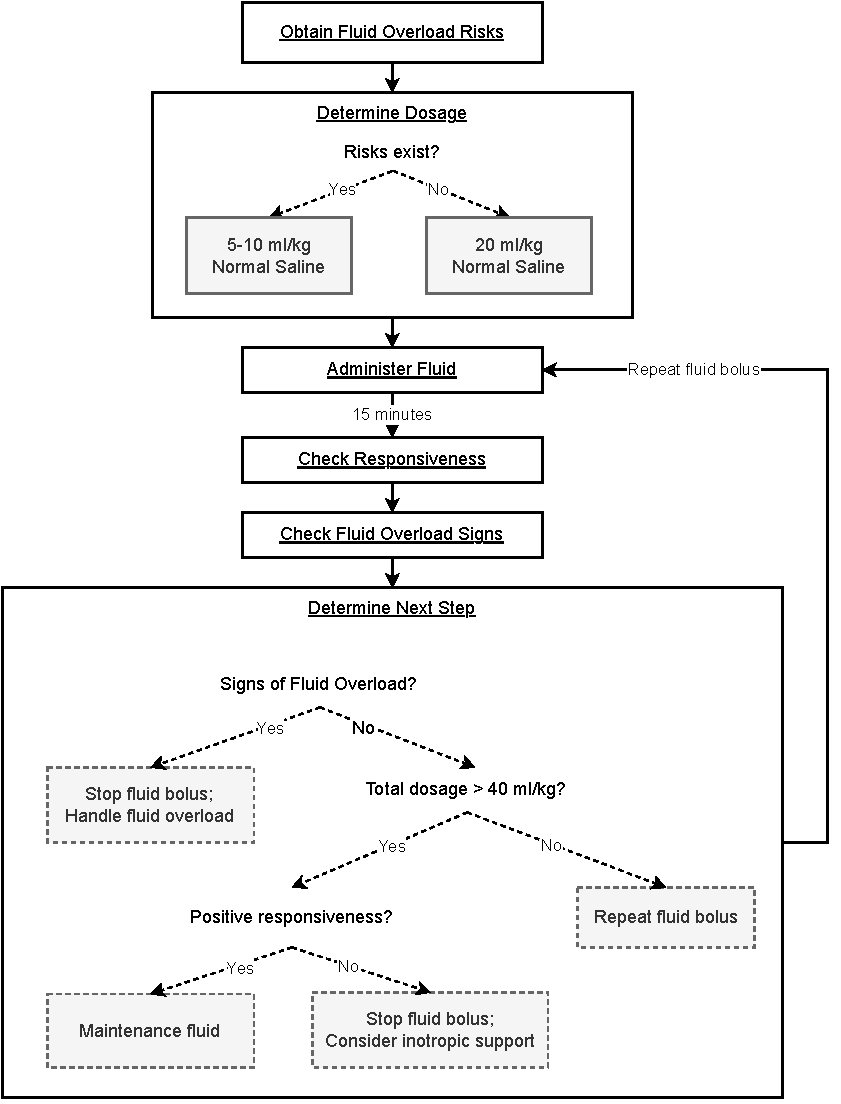
\includegraphics[scale=0.45]{FluidWorkflow-fmcad.pdf}
  \caption{Fluid Resuscitation Guideline}\label{fig:fluid-therapy}
\end{figure}

This real-world \BPG{} exhibits characteristics common
across many \BPGs{}. Specifically \BPGs{} typically:
\begin{itemize}
  \item Involve \stress{concurrent} workflows, such as administering drugs,
    monitoring vitals, performing treatment, etc. There may also be
    inter-workflow interactions. For instance, a diagnosis of sepsis during the
    screening may require modifications to an ongoing course antibiotics.
  \item Often specified in a \stress{flowchart-like}
    notation. See \cite{AHAFlowcharts} and \cite{CancerCareFlowcharts} for other flowchart-based \BPGs{} for management of \emph{cardiac arrest}, and
    screening, risk-reduction, treatment and survivorship in
    cancer care respectively.
  \item Require communication between \stress{heterogeneous agents} such as
     monitors and Electronic Health Records (EHRs).
  \item Often use \stress{tables} indexed by parameters such as age, weight,
    etc to present normal/abnormal ranges for measurements, or recommended dosages for drugs.
\end{itemize}

\begin{footnotesize}
  \begin{table}
    \centering
    \begin{tabular}{ | c || c | c | c | }
      \hline
      \textbf{Age}            & \textbf{Heart Rate}   & \textbf{Systolic BP} & \textbf{Temp}  \\
      \hline
      $0d - 1m$               & $>205$                & $<60$                & $<36 \text{ or } >38$ \\
      \hline
      $\geq 1m - 3m$          & $>205$                & $<70$                & $<36 \text{ or } >38$ \\
      \hline
      $\geq 3m - 1y$          & $>190$                & $<70$                & $<36 \text{ or } >38.5$ \\
      \hline
      $\dots$                 & $\dots$               & $\dots$              & $\dots$ \\
      \hline
      $\geq 13y$              & $>100$                & $<90$                & $<36 \text{ or } >38.5$ \\
      \hline
    \end{tabular}
    \caption{Vital Signs Chart}\label{table:vital-signs}
  \end{table}
\end{footnotesize}

Note that the aforementioned characteristics are \emph{not} specific
to one guideline. According to a review paper on \CIGs{} \cite{ClerqAIM03},
such \DSLs{} should additionally
\begin{enumerate*}[label=(\alph*)]
  \item be formally defined, i.e, have a formal syntax and semantics, and
  \item have an execution engine to provide decision support.
\end{enumerate*}


%In the following sections, we describe how these characteristics dictate the
%design philosophy behind \MediK{}. We argue that this philosophy
%makes \MediK{} both intuitive to \HCPs{}, and suitable for expressing
%complex guidelines.

